\chapter{Methods}




All analyses were done in R version 3.4.3 (2017-11-30) on an x86\_64-pc-linux-gnu (64-bit) 
running Ubuntu 16.04.4 LTS. 
Complex survey designs of the NIS and NRD  were accounted for using the \texttt{survey} package, version 
3.33-2 \cite{Lumley2018}. Data were stored and retrieved in
MonetDB using MonetDBLite version 0.5.1 \cite{Muehleisen2018}.

\section{Data source}

Years 2001-2014 of the NIS, as well as years 2010-2014 of the NRD were provided courtesy of Creighton University
School of Medicine. Both datasets originate in comma-separated variables (CSV) format. 

The NIS covers between 7-8 million unweighted patients per calendar year, resulting in file sizes around 3 GB on average,
totaling around 43 GB of raw ASCII text.

\begin{lstlisting}[language=Bash]
  $ l -ha NIS* | awk '{print $5, $9}'
  2.7G NIS2001.csv                                                          
  2.9G NIS2002.csv                                                          
  3.0G NIS2003.csv                                                          
  3.1G NIS2004.csv                                                          
  3.1G NIS2005.csv                                                          
  3.1G NIS2006.csv                                                          
  3.4G NIS2007.csv                                                          
  3.4G NIS2008.csv                                                          
  3.5G NIS2009.csv
  3.6G NIS2010.csv
  3.7G NIS2011.csv
  2.6G NIS2012.csv
  2.6G NIS2013.csv
  2.8G NIS2014.csv
\end{lstlisting}

The NRD is normalized into 4 different files, 3 discharge-level files and a hospital-level file.

The \texttt{Core} file contains data elements necessary for readmission analysis. The \texttt{Severity} files
contain data related to the severity of the patients' conditions, including, for our purposes, comorbidity flags.
The \texttt{DX\_PR} file (diagnoses and procedures) file contains ICD-9-CM codes and other fields related to
diagnoses and procedures. Finally, the hospital file contains information on the hospital characteristics.

The NRD is a record of around 14 million unweighted admissions per calendar year with identifiers that allow analysts 
to track readmissions from a particular index event.

\centering
\begin{lstlisting}[language=Bash]
  $ l -ha NRD*/*.CSV | awk '{print $5, $9}' | sed -e 's/ /\t/'
  5.0G    NRD2010/NRD_2010_Core_V2.CSV
  3.4G    NRD2010/NRD_2010_DX_PR_GRPS_V2.CSV
  88K     NRD2010/NRD_2010_Hospital_V2.CSV
  1.2G    NRD2010/NRD_2010_Severity_V2.CSV
  5.1G    NRD2011/NRD_2011_Core_V2.CSV
  3.4G    NRD2011/NRD_2011_DX_PR_GRPS_V2.CSV
  87K     NRD2011/NRD_2011_Hospital_V2.CSV
  1.2G    NRD2011/NRD_2011_Severity_V2.CSV
  4.9G    NRD2012/NRD_2012_Core_V2.CSV
  3.3G    NRD2012/NRD_2012_DX_PR_GRPS_V2.CSV
  82K     NRD2012/NRD_2012_Hospital_V2.CSV
  1.1G    NRD2012/NRD_2012_Severity_V2.CSV
  5.2G    NRD2013/NRD_2013_Core.CSV
  3.4G    NRD2013/NRD_2013_DX_PR_GRPS.CSV
  92K     NRD2013/NRD_2013_Hospital.CSV
  1.1G    NRD2013/NRD_2013_Severity.CSV
  6.6G    NRD2014/NRD_2014_Core.CSV
  4.1G    NRD2014/NRD_2014_DX_PR_GRPS.CSV
  98K     NRD2014/NRD_2014_Hospital.CSV
  1.2G    NRD2014/NRD_2014_Severity.CSV
\end{lstlisting}
\label{fig:nrd-size} 
\caption{blah}

This totals to over 50 GB of raw ASCII text. 

\subsection{Persistence}

There are numerous ways to handle a dataset of this size. If we know exactly what unique codes we want,
we could simply \texttt{grep} for them. However, this isn't scalable and we would not be able to calculate
population proportions.

For this project, we imported the data into MonetDBLite, an in-process version of MonetDB. 
We chose MonetDB, because it fits well in the academic space, being open source with strong R 
integration and good community support.
It also fits well in the data warehousing space, being a pioneer in column-store technologies. 

Column-store databases partition each column as an array, making data retrieval extremely fast when
only a subset of the columns need to be loaded into memory \cite{MonetDB}.

\subsection{Diagnosis and procedure codes}

The International Classification of Diseases, Ninth Revision, Clinical Modification (ICD-9-CM) is based on the World Health Organization's Ninth Revision,
International Classification of Diseases (ICD-9). It is the coding standard for diseases and procedures used in the NIS and NRD up to October, 2015, when
HCUP upgraded to ICD-10-CM. 

Although we had access to the 2015 NRD data, it was not used due to the added complexity of accounting for ICD-10-CM changes, as well as not having 2015
data for NIS, which would have caused inconsistencies in trend analysis. 

With the acknowledgement that ICD-9-CM codes are not perfect \cite{Uchiyama2015}, they are still the best thing we have for longitudinal 
epidemiological studies on a large scale. 

All diagnosis fields, \texttt{dx1, dx2,} $\hdots$ \texttt{dx30} were queried for code \textbf{00845} (\textit{Intestinal infection due to Clostridium difficile}). 
The decision not to look exclusively at \texttt{dx1}, the principal diagnosis, was deliberate, due to the nature of CDI. Patients rarely contract CDI
independently. It is typically contracted while in a hospital setting while being treated for a separate disease. 

To complicate matters, ICD-9-CM codings are not an exact science, and are often done based on cost and seriousness of comorbid conditions. Coders must use
their judgement for determining a principal diagnosis when comorbid conditions are present \cite{Avery2011}. For this reason, we simply simply queried for
the presence of the condition on any diagnosis field. 

The same was done for renal failure codes.

\begin{table}[]
\centering
\caption{ICD-9-CM renal failure codes}
\label{icd9renal}
\begin{tabular}{ll}
Code  & Description          \\
\hline
584   & Acute kidney failure \\
584.5 &	Acute kidney failure with lesion of tubular necrosis convert \\
584.6 &	Acute kidney failure with lesion of renal cortical necrosis convert \\
584.7 &	Acute kidney failure with lesion of renal medullary [papillary] necrosis \\
584.8 &	Acute kidney failure with lesion of with other specified pathological lesion in kidney \\
584.9 &	Acute kidney failure, unspecified \\
585   & Chronic kidney disease (ckd) \\
585.1 &	Chronic kidney disease, Stage I \\
585.2 &	Chronic kidney disease, Stage II (mild) \\
585.3 &	Chronic kidney disease, Stage III (moderate) \\
585.4 &	Chronic kidney disease, Stage IV (severe) \\
585.5 &	Chronic kidney disease, Stage V (mild) \\
585.6 &	End stage renal disease \\
585.9 &	Chronic kidney disease, unspecified \\
586   &	Renal failure, unspecified \\
\end{tabular}
\end{table}

For trend analysis, the CDI and renal failure selections were joined. This provided full samples of
CDI and renal patients, as well as patients with both.


\subsection{Determining index admissions and readmissions}

Unlike the NIS, the NRD allows tracking patients across hospital visits within a given calendar year.
The field \texttt{nrd\_visitlink} provides a key that identifies a single patient across multiple visits.
To determine temporality, a length of stay field (\texttt{los}) is provided for each visit, as well as
a reference date, \texttt{nrd\_daystoevent}. To ensure anonymity, a randomly selected date is chosen for 
each patient. \texttt{nrd\_daystoevent} then references the random date and lists the days from the epoch date.
This way, no precise date can be determined, thereby protecting patient privacy, while providing the researcher
with the data he or she needs. 

The NRD leaves readmission determination up to the analyst. First an index event must be chosen. 
We selected all cases of CDI (ICD-9-CM code \textbf{00845}) and retrieved all unique \texttt{nrd\_visitlink}
identifiers. Then a second query was performed retrieving all events for the \texttt{nrd\_visitlink} identifiers.

We then grouped the cases first by \texttt{nrd\_visitlink}, then chronologically. Then, we scanned for the first
occurrence of a CDI event (ICDM-9-CM code \textbf{00845}) and marked it as the index event. All information from
the index event was stored in a "patient profile" object. The remaining patient admissions, if any, were scanned.
If the event contained a CDI identifier and fell within the given readmission day window (30, 60, and 90 days, separately),
the event was considered a readmission and the number of readmissions were stored. If the patient died on a readmission,
that was also stored. If the secondary event fell outside of the readmission window, it was considered another index event, 
and the process started over.

The following additional rules were applied for determining index events for \textit{d}-day readmissons, where $d = \{30, 60, 90\}$:

\begin{enumerate}
    \item For years 2010-2014: ($1 \le \text{DMONTH} \le 12 - ceil(d/30)$)
    
    We needed to cut off index events with enough time to determine if there was a readmission, since only calendar years can be analyzed.
    
    \item $\text{DIED} \ne 0$
    
    A death on index does not allow for readmission.
    
    \item $\text{LOS} > 0$
    
    A length of stay equal to zero represents transfers and same-day stays that were combined which represents a more complex type of care \cite{NRDIntroduction2013}.
    
    \item $AGE > 0$
  
    About 70\% of infants under one year of age carry \cdiff without showing signs or symptoms of infection \cite{Lamont2017}. 
    
\end{enumerate}



\begin{figure}[h]
\centering
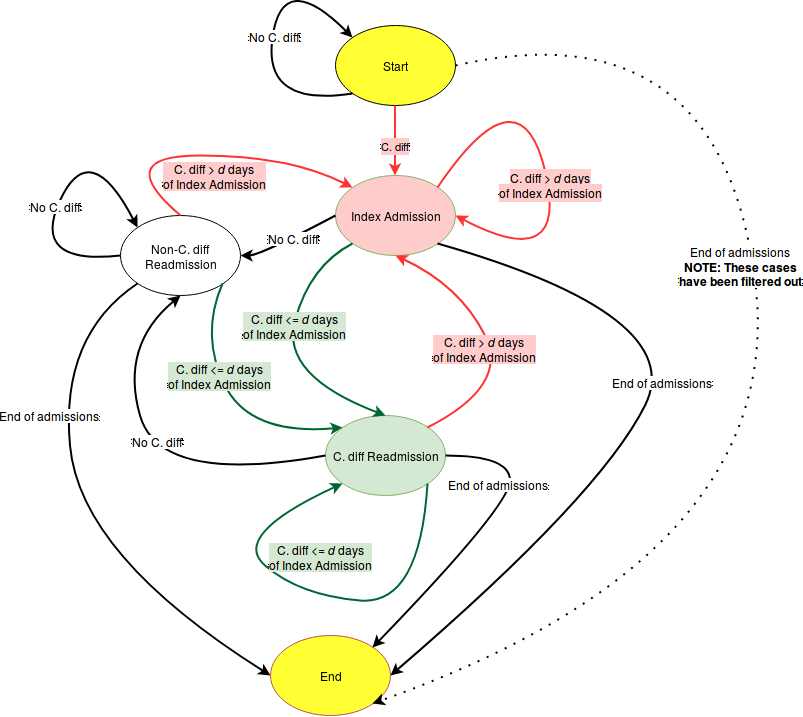
\includegraphics[scale=0.5]{readmission-state-diagram.png} 
\label{fig:readmission-state-diagram} 
\caption{State diagram for determining what constitutes an index admission and a subsequent readmission.
Additional rules include cutting off index events by October, November, or December, depending on whether we are looking for 90, 60, 30 day readmissions, respectively;
filtering out deaths on index events;
lengths of stay that included transfers and same-day stays;
and infants less than 1 year of age, where \cdiff bacteria are common but the patient shows no symptoms.}
\end{figure}


\subsection{Choosing features}

To determine renal failure comorbidities, the \texttt{cm\_renlfail} flag was first used, and then more specific ICD-9-CM codes were identified. Acute kidney failure, 
or acute kidney injury (AKI) were grouped by all sub-category codes into a single AKI category. This included codes \textbf{584}, \textbf{584.5}, \textbf{584.6}, \textbf{584.7}, 
\textbf{584.8}, and \textbf{584.9}. 

Chronic kidney disease (CKD) stages were individually analyzed, but unspecified or unknown CKD cases were grouped, (ICD-9-CM codes \textbf{585} and \textbf{585.9}). 

Additionally, we considered hospital characteristics as independent factors, including hospital control (Government, nonfederal; Private, non-profit; Private, invest-own), 
urban/rural designation (9 categories from smallest to largest), teaching designation, and bedsize. 

Hospital urban/rural designations contained 9 categories 1 being the largest and 9 being the smallest. These were reversed in order to have a meaningful effect in the regression.

Sex was also included in the regression.

Patients' age is included in the eGFR formula, and as such, would be a confounding variable, so it was not included in the regression.

\section{Statistical analysis}

Descriptive and inferrential statistics were done using the NIS and NRD complex survey design, 
supplying \texttt{hospid} as the clusters, \texttt{nis\_stratum} as the strata, and \texttt{discwt} as the weighting. 
Lonely primary sampling units (PSU) - in our case, hospitals - were excluded using \texttt{options(survey.lonely.psu="remove")} \cite{LonelyPSUs}.

The primary readmission analysis was done with multivariable logistic regression to determine the effect of the covariates and confounding variables
on the likelihood of being readmitted with CDI under the three readmission windows, 30, 60, and 90 days. 

The model was fitted independently on each year's data. 
We could have included the years as independent variables and attempted to fit the entire dataset, but we chose not to. The primary reason being, the dataset is very large,
so a single all-year fit was somewhat impractical due to hardware resource limitations. More academically, however, we are able to capture more nuance in modelling individual
years, given each year is a separate independent data set, and medical trends do change over time. Fitting 5 years of data all at once, is likely to miss smaller subtleties, 
such as increases or decreases in a particular coefficient over time. 

Variance estimation was done using Jackknife Repeated Replication (JRR), specifically the JKn approach. Replication methods have shown better
precision and reduced bias compared to Taylor Series Linearization \cite{Chowdhury2013, Smith2000}.

All charts were done with the \texttt{ggplot2} package. 
